\section{Α.Α.Μ. σε βάθος}
\selectlanguage{greek}
Ο Αλγόριθμος Αποικίας Μυρμηγκιών (Α.Α.Μ.) είναι ένας μετευρετικός αλγόριθμος βελτιστοποίησης που έχει ως στόχο την εύρεσης βέλτιστης διαδρομής σε κάποιο πρόβλημα. Μετευρετικούς ονομάζουμε τους αλγόριθμους που είναι βασισμένοι σε ευφυείς επαναληπτικές τεχνικές και αντί να ακουλουθούν έναν αυστηρό κανόνα εξάγουν γνώση με τρόπους που είναι εμπνευσμένοι από συμπεριφορές στην φύση. \cite{ribeiro2002ant} Συγκεκριμένα, ο Α.Α.Μ. είναι βασισμένος στην συμπεριφορά τον μυρμηγκιών για την αναζήτηση τροφής. 
Τα μυρμήγκια έχουν την ικανότητα να βρίσκουν πάντα την βέλτιστη διαδρομή προς την πηγή τροφής όσο δύσκολο κι αν είναι αυτό. Κατά συνέπεια κι ο Α.Α.Μ. είναι ικανός να βρει ικανοποιητικές λύσεις σε περίπλοκα προβλήματα και να εξερευνήσει μεγάλους χώρους αναζήτησης σε μικρό χρονικό διάστημα. Όπως αναφέρθηκε και στο προηγούμενο κεφάλαιο, όταν τα μυρμήγκια κινούνται στο χώρο αφήνουν φερομόνη. Αυτή η ουσία αποτελεί και τρόπο επικοινωνίας μεταξύ των μυρμηγκιών, για εύρεση βέλτιστης διαδρομής προς την τροφή, αφού όσο περισσότερη φερομόνη υπάρχει σε μία διαδρομή, τόσο αυξάναται κι η πιθανότητα ένα επόμενο μυρμήγκι να ακολουθήσει αυτή τη διαδρομή. 


\subsection{Βασική Θεωρία}
Τα τεχνητά μυρμήγκια που χρησιμοποιούνται στον Α.Α.Μ. είναι εμπνευσμένα από την συμπεριφορά των πραγματικών μυρμηγκιών και αποτελούν διαδικασίες κατασκευής στοχαστικών λύσεων που με χρήση πιθανολογικών τεχνικών και χρησιμοποιόντας μία δυναμική δομή μνήμης που συσχετίζεται με την ποιότητα της λύσης του προηγούμενου ληφθέντος αποτελέσματος επιλύουν υπολογιστικά προβλήματα, όπως αυτό της εύρεσης βέλτιστου μονοπατιού μέσω γράφων, προσθέτοντας επαναληπτικά στοιχεία σε επιμέρους λύσεις λαμβάνοντας υπόψη ευρετικές πληροφορίες σχετικά με την επίλυση του προβλήματος και (τεχνητές) διαδρομές φερομόνης που αλλάζουν δυναμικά στο χρόνο εκτέλεσης. \cite{dorigo2003ant} \cite{mavrovouniotis2017survey}

\subsection{Μαθηματικό υπόβαθρο}

\selectlanguage{english}
\begin{figure}[ht]
    \begin{minipage}[c]{.46\linewidth}
        \centering
        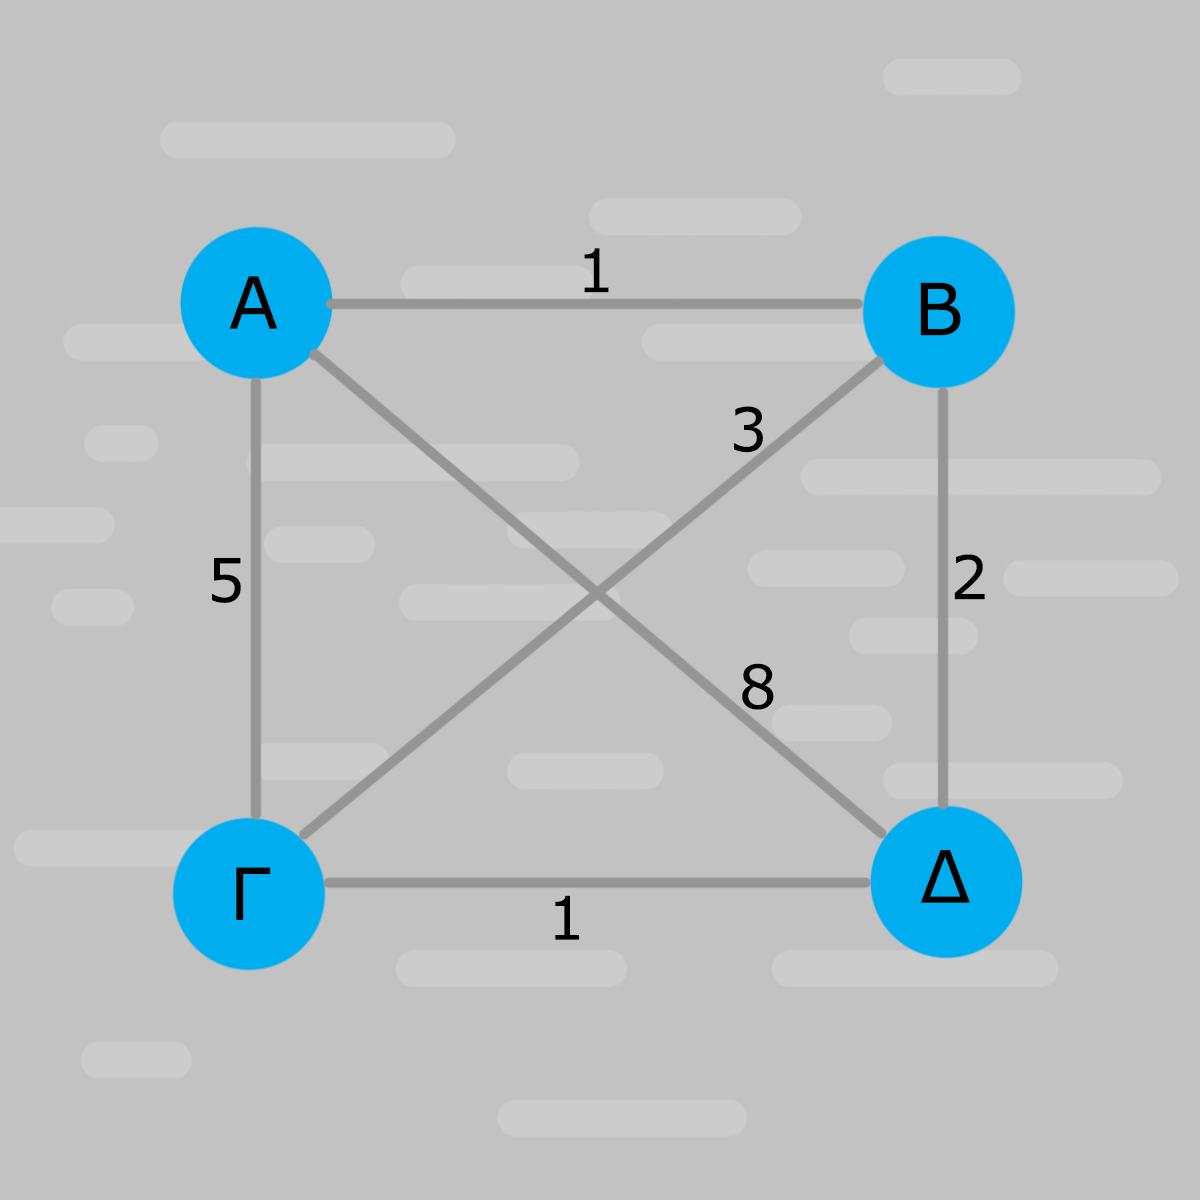
\includegraphics[scale=0.15]{2947_thesis/pictures/apostaseis.png}
        \caption{Απόσταση}
        \label{distance}
    \end{minipage}
    \begin{minipage}[c]{.46\linewidth}
        \centering
        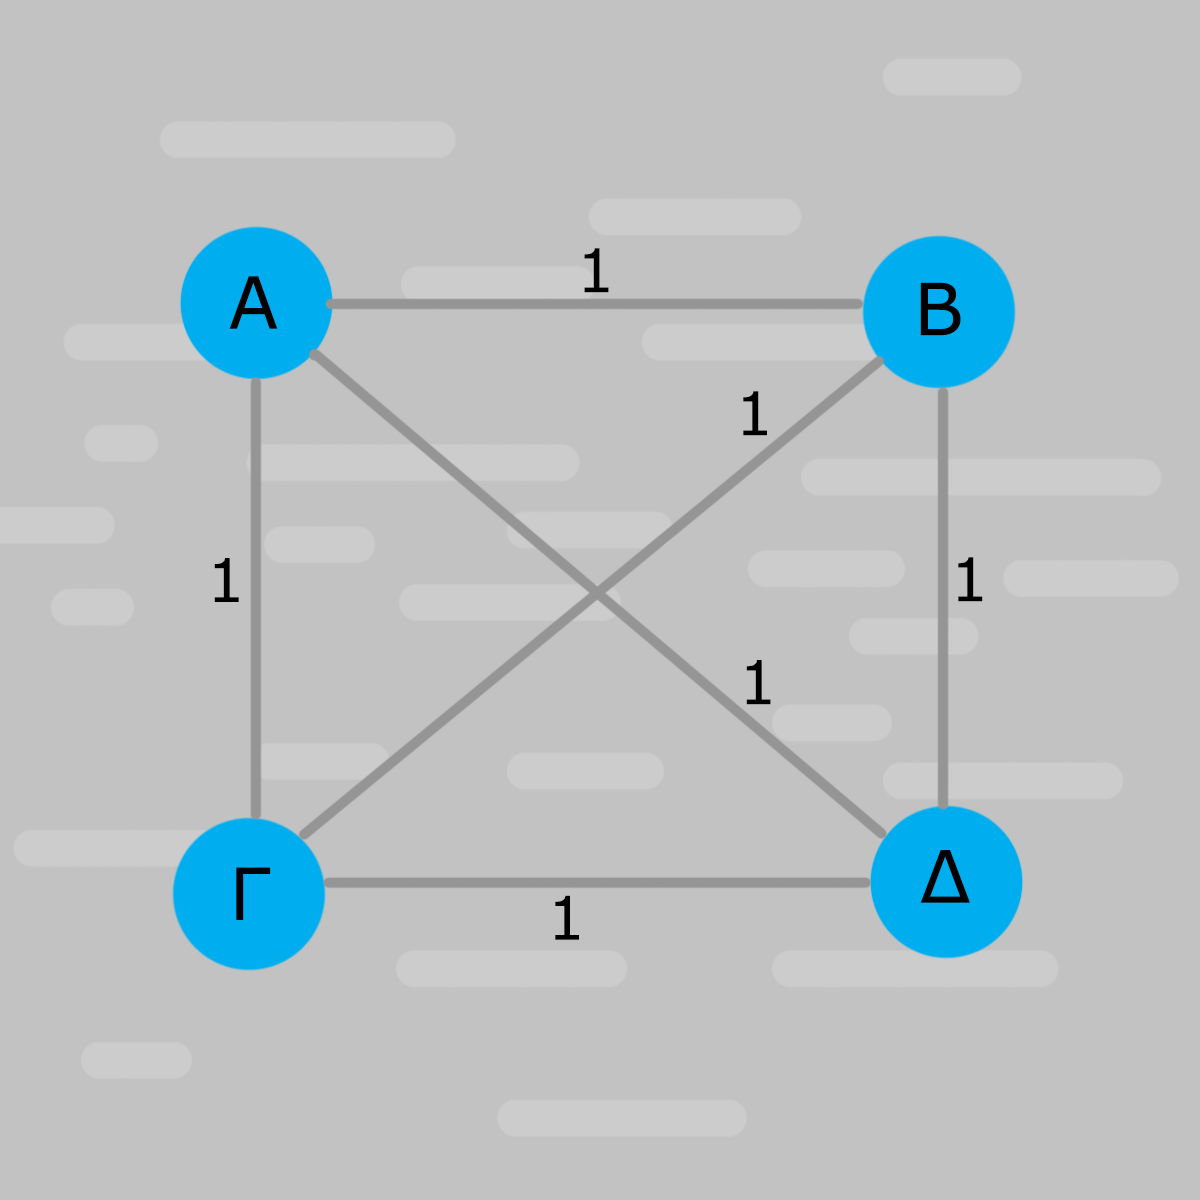
\includegraphics[scale=0.15]{2947_thesis/pictures/feromoni.png}
        \caption{Φερομόνη}
        \label{pher}
    \end{minipage}
\end{figure}
\subsubsection{Απόσταση}
Όπως αναφέρθηκε και στην δεύτερη ενότητα, ο γράφος είναι ένα απαραίτητο κομμάτι για τη μοντελοποίηση προβλημάτων με χρήση του αλγόριθμου αποικίας μυρμηγκιών. Η απόσταση, όπως και η φερομόνη, θα μοντελοποιηθούν με χρήση αναπαράστασης πίνακα. Κάθε ακμή του γράφο έχει ένα κόστος που συμβολίζει την απόσταση ή την γενικότερη ποιότητα της διαδρομής μεταξύ δύο κορυφών. Έστω οι κορυφές Α, Β, Γ, Δ που ενώνονται μεταξύ τους όπως φαίνεται στο [Figure \ref{distance}] το οποίο αποτυπώνεται σε πίνακα γειτνίασης ως εξής:
$$
Distance = 
 \begin{array}{c|c c c c}
    & A & B & Γ & Δ \\ \hline
    A & 0 & 1 & 8 & 5 \\
    B & 1 & 0 & 2 & 3 \\
    Γ & 8 & 2 & 0 & 1 \\
    Δ & 5 & 3 & 1 & 0 
 \end{array}
 $$
 Πρόκειται για έναν μη κατευθυνόμενο γράφο, δηλαδή συμμετρικό πίνακα και έχει βάρη σε κάθε ακμή που υποδηλώνουν το κόστος επιλογής της κάθε διαδρομής, είτε αυτό εκφράζεται ως απόσταση, είτε με κάποιον άλλο τρόπο.
\subsubsection{Φερομόνη}
Τα μυρμήγκια αφήνουν φερομόνη από όπου περνούν ανάλογα με την ποιότητα της λύσης που βρήκαν. Σε καλύτερες λύσεις συσσωρεύεται περισσότερη φερομόνη από τις υπόλοιπες. Τα μονοπάτια φερομόνης εκφράζονται ως αριθμητικές πληροφορίες μέσω ενός πίνακα, που χρησιμοποιούν τα επόμενα μυρμήγκια για την κατασκευή πιθανών λύσεων στο εκάστοτε πρόβλημα και οι οποίες πληροφορίες μεταβάλονται κατά την εκτέλεση του αλγορίθμου με στόχο της εύρεση του βέλτιστου μονοπατιού. \cite{dorigo2003ant} Σε μονοπάτια που το μυρμήγκι επιστρέφει σε σύντομο χρονικό διάστημα συσσωρεύεται περισσότερη φερομόνη από άλλα μονοπάτια. Υπάρχουν μοντέλα που παράγωγουν περισσότερη φερομόνη ανάλογα με την ποιότητα αυτής της διαδρομής (για παράδειγμα την απόσταση, την ποσότητα της τροφής, και άλλα)
 
Το μαθηματικό μοντέλο αναπαράστασης της φερομόνης που εξάγει το κ-οστό μυρμήγκι στην ακμή που ενώνει τις κορυφές i και j (δηλαδή η ποσότητα της φερομόνης που παράγει) είναι αντιστρόφος ανάλογη με την απόσταση και προκύπτει από τον τύπο:

\begin{align}
	Δτ^k_{i,j}=\frac{1}{L_k}
\end{align}
Όπου:
\begin{itemize}
    \item $L_k$: Η ποιότητα της διαδρομής που βρήκε το μυρμήγκι
\end{itemize}
Έστω ότι για το πρώτο μυρμήγκι είναι παντού 1 [Figure \ref{pher}]. Με αποτέλεσμα να είναι τυχαία η επιλογή διαδρομής. Στο παράδειγμα μας προκύπτει ο πίνακας: 
$$
Pheromone = 
 \begin{array}{c|c c c c}
    & A & B & Γ & Δ \\ \hline
    A & 0 & 1 & 1 & 1 \\
    B & 1 & 0 & 1 & 1 \\
    Γ & 1 & 1 & 0 & 1 \\
    Δ & 1 & 1 & 1 & 0 
 \end{array}
 $$
Οπότε ως έδώ έχουμε ένα χάρτη με τις πιθανά μονοπάτια στον πίνακα distance και το αντίστοιχο κόστος της κάθε διαδρομής και έναν ακόμα με την "επιθυμία" του μυρμηγκιού να επιλέγει το κάθε μονοπάτι στον πίνακα pheromone.

Για να υπολογίσουμε την ποσότητα φερομόνης από μια κορυφή σε μία άλλη (χωρίς εξασθένση- θα αναλυθεί παρακάτω) υπολογίζουμε το άθροισμα της φερομόνης που εξήγαγαν τα μυρμήγκια m που πέρασαν από την κορυφή i στην j. Δηλαδή: 
\begin{align}
    τ_{i,j}^k=\sum_{k=1}^{m}{Δτ^k_{i,j}}
\end{align}

\begin{figure}
    \centering
    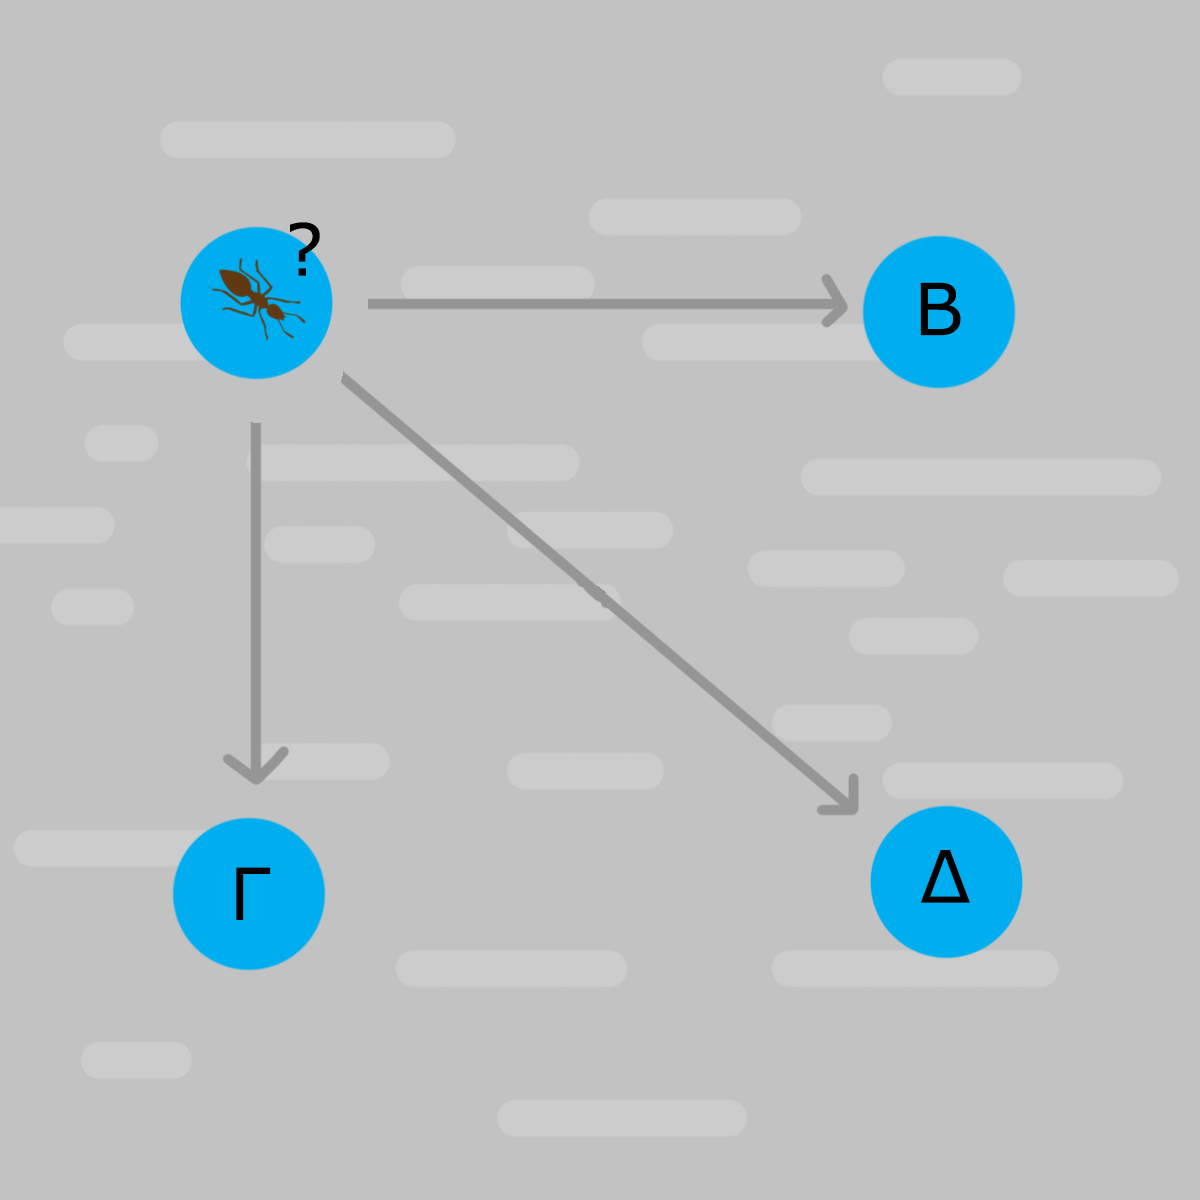
\includegraphics[scale=0.20]{2947_thesis/pictures/epilogi.png} 
    \caption{Πιθανές επιλογές}
    \label{10}
\end{figure}

\subsubsection{Επιλογή Διαδρομής}
Στο παράδειγμα μας ας υποθέσουμε ότι ένα μυρμήγκι ξεκινάει στην κορυφή Α. Οι πιθανές του επιλογές όπως φαίνεται και στο [Figure \ref{10}] είναι οι Β, Γ, Δ. Ποιά είναι όμως η βέλτιστη; 
Με το μάτι σε ένα τόσο απλό πρόβλημα είναι εύκολο να αντιληφθούμε ποιά διαδρομή πρέπει να ακολουθήσει το μυρμήγκι, όμως αυτό δεν είναι εφικτό σε πιο περίπλοκα προβλήματα με μεγάλο αριθμό κορυφών. Έστω ότι ο αριθμός των κορυφών είναι n τότε επιλέγοντας μία κορυφη ως αρχική ο αριθμός των πιθανών κορυφών γίνεται n-1. Αφού το μυρμήγκι επιλέξει μία από αυτές μετά θα αφαιρεθεί από τις πιθανές αφού την επισκέφθηκε και θα γίνουν n-2. Έτσι θα επιλέγει μονοπάτια μεχρι να μην μείνει κανένα διαθέσιμο και να επιστρέψει στο αρχικό. Άρα ο αριθμός των πιθανών επιλογών είναι (n-1)(n-2)(n-3)...3*2*1 = (n-1)!. Όμως δεδομένου ότι διαδρομές όπως Α->Β->Γ->Δ->Α είναι ίδια με την Α->Δ->Γ->Β->Α πρέπει να μην επαναλαμβάνονται. Οπότε αφού πρόκειται για συμμετρικό πρόβλημα ο τύπος των πιθανών μονοπατιών γίνεται είναι $(n-1)!/2$ αφαιρώντας τις επαναλαμβανόμενες λύσεις όπως και στο πρόβλημα του πλανόδιου πωλητή που θα δούμε παρακάτω. 
Η πιθανότητα το κ-οστό μυρμήγκι να επιλέξει μια διαδρομή συμβολίζεται ως: $P^k_{i,j}$ και δίνεται από τον τύπο: \cite{chandrashekar2023hwacoa}

\begin{align} \label{eq:3}
	P^k_{i,j}=\frac{(τ_{i,j})^α(η_{i,j})^β}{\sum_{m}(τ_{i,m})^α(η_{i,m})^β}
\end{align}

Όπου: 
\begin{itemize}
    \item $τ_{i,j}$: το επίπεδο φερομόνης μεταξύ των κορυφών i και j
    \item $η_{i,j}$: η ποιότητα της διαδρομής
    \item m: οι υπόλοιπες διαδρομές που μπορούσε να επιλέξει το μυρμήγκι
    \item α, β: σταθερές που επιλέγουμε ανάλογα από την επιρροή που θέλουμε να έχει το τ και το η στην διαδικασία επιλογής. (Για παράδειγμα αν θέλουμε να επιλέξουμε μια διαδρομή βασισμένη αποκλιστικά και μόνο στο επίπεδο της φερομόνης τότε αφαιρούμε από την εξίσοση το $η_{i,j}$ θέτοντας το β=0).
\end{itemize}
Το γινόμενο των $τ_{i,j}*η_{i,j}$ μας δίνει την "επιθυμία" του μυρμηγκιού να επιλέξει το μονοπάτι i,j.
Στις περισσότερες βιβλιογραφίες αυτή η πιθανότητα αναφέρετε έτσι με διαφορετικούς συμβολισμούς στην καθεμία. 

Στο παράδειγμα μας, αφού υπολογίσουμε την επιθυμία του μυρμηγκιού να επιλέξει την κάθε διαδρομή έχουμε:

\begin{itemize}
    \item AΒ $= τ_{A,B}η_{A,B}=1*\frac{1}{1}=1$ 
    \item AΓ $= τ_{A,Γ}η_{A,Γ}=1*\frac{1}{5}=0.2$
    \item AΔ $= τ_{A,Δ}η_{A,Δ}=1*\frac{1}{8}=0.125$
\end{itemize}

Όπου οι αντίστοιχες πιθανότητες γίνονται:

\begin{itemize}
    \item $P_{A,B}=\frac{1}{1+0.125+0.2}=\frac{1}{1.325}=0.76$
    \item $P_{A,Γ}=\frac{0.2}{1.325}=0.15$
    \item $P_{A,Δ}=\frac{0.125}{1.325}=0.09$
\end{itemize}

Βλέπουμε ότι πιο πιθανό είναι το μυρμήγκι να επιλέξει την διαδρομή ΑΒ όμως υπάρχει πιθανότητα να επιλέξει και τις υπόλοιπες, για την επιλογή της περιοχής χρησιμοποιώντας την πληροφορία που αντλούμε από αυτές τις πιθανότητες, αντί να χρησιμοποιήσουμε μόνο την εντολή random που μας παρέχει η python για τυχαία επιλογή θα χρησιμοποιήσουμε την τεχνική roulette wheel \cite{lipowski2012roulette}. Υπολογίζουμε το άθροισμα συσσωρευμένο, αφού πρόκειτε για πιθανότητα το άθροισμα τους είναι 1, γίνεται η τυχαία επιλογή ενός αριθμού από το 0 έως το 1 και βρίσκουμε το σύνολο στο οποίο αντιστοιχεί αυτός ο αριθμός.
Στην υλοποίησή μου η εντολή: \verb|roulette_wheel_select()| θα επιλέγει μία πόλη τυχαία με βάση τις πιθανότητες. Ο κώδικας που υλοποιεί αυτήν την διαδικασία είναι ο παρακάτω: 
\lstinputlisting[language=python]{code/roulette_wheel.py}
Όπου:
\begin{itemize}
    \item \verb|random_prob|: ένας τυχαίος αριθμός με τον οποίο θα επιλέξουμε περιοχή που θα πάει το μυρμήγκι.
    \item \verb|current|: ο δείκτης τον περιοχών.
\end{itemize}

Στο παράδειγμά μας από 0 έως 0,76 αντιστοιχεί στην διαδρομή ΑΒ, από το 0,77 εως το 0,91 αντιστοιχεί στην διαδρομή ΑΓ και απο το 0,92 έως το 1 στην διαδρομή ΑΔ. Οπότε αν για παράδειγμα επιλεγόταν ο αριθμός 0,41 θα πηγαίναμε στην διαδρομή ΑΒ. [Figure \ref{roulette}]
 
\begin{figure}
    \centering
    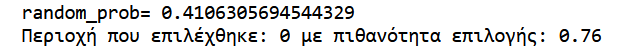
\includegraphics[scale=1]{2947_thesis/pictures/roulette_wheel_example.png} 
    \caption{Παράδειγμα roulette wheel}
    \label{roulette}
\end{figure}


\subsubsection{Εξασθένιση Φερομόνης}

Η διαδικασία της εξασθένισης φερομόνης είναι ένα σημαντικό κομμάτι για την απόδοση του αλγόριθμου και την εύρεση της βέλτιστης λύσης. Όταν όλα τα μυρμήγκια έχουν ολοκλρώσει την διαδρομή τους, ο πίνακας με τις φερομόνες πρέπει να ανανεωθεί. Αυτό γίνεται μέσω εξασθένισης της φερομόνης με ένα στραθερό ρυθμό ρ που καθορίζουμε εμείς. Ένα υψηλο ρ υποδηλώνει γρήγορη εξασθένιση ενώ ένα χαμηλό ρ αργή. Το πόσο γρήγορα εξασθενεί η φερομόνη επηρεάζει τη συμπεριφορά των μυρμηγκιών σε μεγάλο βαθμό. \cite{dawson2013improving} Εμείς θα έχουμε ρ=0.5. (Όπως πρότεινεται από τους Dorigo and Stutzle) \cite{dorigo2003ant} Ο τύπος της εξασθένισης είναι: 

\begin{align}
	τ_{i,j}\leftarrow(1-ρ)τ_{i,j}.
\end{align}

Αυτό επιτρέπει σε λύσεις που δεν είναι ιδανικές να μην λαμβάνονται υπόψην. Όπως αναφέρθηκε και στο κεφάλαιο 3.2.2 ο τύπος για τον υπολογισμό της φερομόνης από μία κορυφή σε μία άλλη είναι: 
\begin{align}
    τ_{i,j}^k=\sum_{k=1}^{m}{Δτ^k_{i,j}}
\end{align}
Με εξασθένιση αυτός γίνεται: 
\begin{align}
    τ_{i,j}^k\leftarrow(1-ρ)τ_{i,j}+\sum_{k=1}^{m}{Δτ^k_{i,j}}
\end{align}
Όπου: 
\begin{itemize}
    \item $τ_{i,j}$ η ποσότητα της φερομόνης στην προηγούμενη επανάληψη
    \item 1-ρ ο ρυθμός εξασθένισης
    \item $\sum_{k=1}^{m}{Δτ^k_{i,j}}$ το άθροισμα φερμόνης που άφησαν όλα τα μυρμήγκια m που πέρασαν από αυτή την περιοχή
\end{itemize}

\subsubsection{Διάγραμμα Αλγορίθμου}


\subsection{Υλοποίησή μου Αλγορίθμου σε python}
Αφού κάνουμε import τις απαραίτητες βιβλιοθήκες, αρχικοποιούμε τις μεταβλητές που θα χρειαστούμε. Αυτές είναι ο αριθμός των περιοχών που μπορούν να επισκεφτούν τα μυρμήγκια (areas), ο αριθμός των μυρμηγκιών (ants), ο αριθμός των επαναλήψεων που θα εκτελεστεί ο αλγόριθμος (iterations) και οι σταθερές α και β (alpha, beta).
\lstinputlisting[language=python]{code/step1.py}

Έπειτα δημιουργούμε τον πίνακα με τον οποίο θα μοντελοποιούμε την ποιότητα της διαδρομής (distance). Αυτό το κάνουμε τυχαία επιλέγοντας έναν αριθμό από το 0 εως το 50 για κάθε ακμή του γράφου.
\lstinputlisting[language=python]{code/step2_1.py}

Πρόκειται για έναν μη κατευθυνόμενο γράφο οπότε πρέπει να τον μετατρέψουμε σε συμμετρτικό, αυτό το κάνουμε προσθέτοντας τον πίνακα distance με τον ανάστροφο πίνακα $distance^{Transposed}$ και διερούμε με το 2, επίσης αφαιρερούμε τους βρόχους (ακμές που ξεκινάν και τελειώνουν στην ίδια κορυφή) θέτοντας 0 στα κελιά (i,i), $i\in[0,areas)$. \cite{perez2020introduction}
\lstinputlisting[language=python]{code/step2_2.py}

Αρχικοποιούμε τον πίνακα με τις φερομόνες (pheromone) να έχει παντού 1. Στην πρώτη επανάληψη του αλγορίθμου η επιλογή διαδρομής από ένα μυρμήγκι θα εξαρτάτε μόνο από τον πίνακα ποιότητας της διαδρομής (distance). 
\lstinputlisting[language=python]{code/step3.py}

Έπειτα για όσες φορές θέλουμε να εκτελέσουμε τον αλγόριθμο (iterations):
τοποθετούμε το κάθε μυρμήγκι σε μια τυχαία περιοχή ως αρχική του, αυτό το κάνουμε δημιουργόντας μια λίστα (ant\_areas) μεγέθους όσα και τα μυρμήγκια και επιλέγοντας μία τυχαία περιοχή για το καθένα με χρήση της randint. \cite{w3school}
\lstinputlisting[language=python]{code/step4_1.py}
Η πάνω διαδικασία μπορεί επίσης να γραφεί ως εξής: 
\lstinputlisting[language=python]{code/step4_2.py}

Στην συνέχεια κάθε μυρμήγκι επιλέγει την επόμενη περιοχή που θα επισκεφτεί για όσες περιοχές υπάρχουν (areas) με χρήση της φερομόνης (pheromone) και του κόστους επιλογής κάθε διαδρομής (distance). Αυτό θα το πετύχουμε μοντελοποιόντας την συνάρτηση (\ref{eq:3}). Η τυχαία επιλογή αριθμού όπως αναφέρθηκε και στο κεφάλαιο 3.2.3 θα γίνεται με την συνάρτηση roulette\_wheel\_select() που δημιουργήσαμε. 
Αρχικά υπολογίζουμε τις διαθέσιμες περιοχές που μπορεί να επισκεφθεί το κάθε μυρμήγκι (available\_areas). Έπειτα υπολογίζουμε την επιθυμία του κάθε μυρμηγκιού να ακολουθήσει κάθε μονοπάτι από τα διαθέσιμα και στη συνέχεια την πίθανότητα επιλογής του κάθε μονοπατιου. Αυτή την πιθανότητα την εισάγουμε ως μεταβλητή στην συνάρτηση roulette\_wheel\_select() που δημιουργήσαμε και έχουμε ως αποτέλεσμα τον δείκτη που βρίσκεται η περιοχή που επιλέχθηκε να ακολουθήσει το μυρμήγκι στον πίνακα με τις διαθέσιμες περιοχές. Αυτό το ονομάζουμε next\_area. Τέλος προσθέτουμε τον πίνακα με τη διαδρομή κάθε μυρμηγκιού στο ant και υπολογίζουμε το μήκος αυτών στο ant\_distances. 
\lstinputlisting[language=python]{code/step5.py}

Έπειτα, αφού έχουμε βέλτιστη λύση από την εκτέλεση του αλγορίθμου, ανανεώνουμε τον πίνακα με τις φερομόνες έτσι ώστε καλύτερες λύσεις να είναι πιο πιθανό να επιλεγούν.
\lstinputlisting[language=python]{code/step6.py}
Όπου το ρ=0.5, ο ρυθμός εξασθένισης και pheromone\_sum το $\sum_{k=1}^{m}{Δτ^k_{i,j}}$. 


Αυτή την διαδικασία την επαναλαμβάνουμε όσες φορές θέλουμε να εκτελεστεί ο αλγόριθμος (iterations). Όσο μεγαλύτερο το iterations, τόσο καλύτερη θα είναι η λύση, αφού κάθε επανάληψη αυξάνει την πιθανότητα να βρεθεί μια ακόμα καλύτερη λύση από την προηγούμενη και έχει ως αποτέλεσμα να πλησιάζουμε όλο και περισσότερο στην βέλτιστη.


\begin{table}
\begin{center}
\begin{tabular}{|c|c|}
    \hline
    {\bf Μεταβλητή} & {\bf Ιδιότητα}\\ \hline
    ants & αριθμός μυρμηγκιών\\ \hline
    areas & αριθμός περιοχών\\ \hline
    iterations & αριθμός επαναλήψεων\\ \hline
    alpha & σταθερά "α"\\ \hline
    beta & σταθερά "β" \\ \hline
    distance & πίνακας μεγέθους areas*areas με\\
    &  κόστος επιλογής κάθε μονοπατιού\\ \hline
    pheromone & πίνακας μεγέθους areas*areas με\\ 
    & ποσότητα φερομόνης σε κάθε μονοπάτι\\ \hline
    ant\_areas & λίστα μεγέθους όσα και τα\\ 
    & μυρμήγκια με αρχικές περιοχές\\
    & για το καθένα\\ \hline
    available\_areas & διαθέσιμες περιοχές που μπορεί\\ 
    & να επισκεφτεί το κάθε μυρμήγκι\\ \hline
    probabilities & η "επιθυμία" επιλογής κάθε\\
    & μονοπατιού από κάθε μυρμήγκι\\ \hline
    total\_pheromone & το άθροισμα όλων των επιθυμιών\\ 
    & κάθε επανάληψης\\ \hline
    next\_area & επιλεχούσα περιοχή με\\ 
    & χρήση roulette\_wheel\_select\\ \hline
    pheromone\_sum & άθροισμα φερομόνης σε κάθε μονοπάτι\\ \hline
    ant\_distances & άθροισμα κόστους διαδρομών\\ 
    & που επέλεξε το κάθε μυρμήγκι\\ \hline
    best\_route & λίστα με καλύτερες διαδρομές\\
    & της κάθε επανάληψης\\ \hline
    best\_one\_route & μονοπάτι καλύτερης διαδρομής\\
    & από όλες τις επαναλήψεις\\ \hline
    best\_one\_distance & κόστος καλύτερης διαδρομής\\ \hline

\end{tabular}
\end{center}
\caption{Πίνακας με μεταβλητές αλγόριθμου}
\end{table}


Παρακάτω δίνετε ο αλγόριθμος ολοκλήρωμένος:
\lstinputlisting[language=python]{code/ant_colony_algorithm.py}



\subsection{Εκτέλεση του Αλγορίθμου}
Στο παράδειγμα που εκτελέσαμε τον αλγόριθμο έχουμε ως δεδομένα 5 μυρμήγκια που εκτελούν αναζήτηση μεταξύ 5 περιοχών 10 φορές με alpha και beta 1, η εκτέλεση του αλγορίθμου με τα παραπάνω δεδομένα δίνουν αποτέλεσμα παρόμοιο με αυτό που φαίνεται στο [Figure \ref{12}].

\begin{figure}
    \centering
    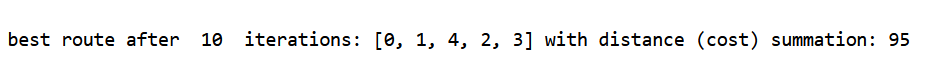
\includegraphics[scale=0.55]{2947_thesis/pictures/ex1.png} 
    \caption{Παράδειγμα με: ants=5, areas=5, iterations=10, alpha=beta=1.}
    \label{12}
\end{figure}

Ανάλογα από τις απαιτήσεις του εκάστοτε προβλήματος, οι μεταβλητές μπορούν να αλλάξουν, τί γίνεται όταν αλλάξουμε τα alpha και beta, τί συμβαίνει με μικρό αριθμό επαναλήψεων, πώς λειτουργεί το πρόγραμμα με εξασθένιση και πώς χωρίς εξασθένιση, πώς σχετίζεται η ποιότητα της λύσης με τον αριθμό των μυρμηγκιών; Ερωτήσεις σαν κι αυτές θα απαντηθούν παρακάτω με παραδείγματα εκτέλεσης του αλγορίθμου και με τα αντίστοιχα αποτελέσματα. 
Για εύκολη κατανόηση του προβλήματος και για τον σκοπό της επίτευξης των συγκρίσεων θα γίνει χρήση ίδιου πίνακα distance σε όλα τα παρακάτω παραδείγματα, ο οποίος δίνεται στο [Figure \ref{13}] με βέλτιστα αποτελέσματα που φαίνονται στο [Figure \ref{14}]
\begin{figure}
    \centering
    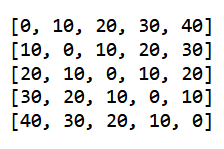
\includegraphics[scale=1]{2947_thesis/pictures/distance.png} 
    \caption{Πίνακας distance που θα χρησιμοποιηθεί για τα παραδείγματα.}
    \label{13}
\end{figure}
\begin{figure}
    \centering
    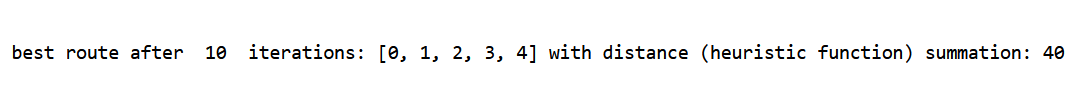
\includegraphics[scale=0.55]{2947_thesis/pictures/ex2.png} 
    \caption{Βελτιστα αποτελέσματα για είσοδο distance του Figure \ref{13}.}
    \label{14}
\end{figure}

\subsubsection{Τροποποίηση των alpha, beta}

Σε περίπτωση που το alpha πάρει την τιμή 0, η επιρροή που έχει ο πίνακας με τις φερομόνες (pheromone) μηδενίζεται, αφαιρόντας έτσι το δυνατότητα του αλγόριθμου να "μάθει" από προηγούμενες εκτελέσεις, με αποτέλεσμα ο αλγόριθμος να βασίζεται μόνο στο πίνακα με το κόστος επιλογής κάθε διαδρομής (distance) και κατά συνέπεια στο ποιό είναι το καλύτερο μονοπάτι εκείνη την χρονική στιγμή χωρίς να δίνεται βάση σε προηγούμενες λύσεις. Το πρόγραμμα μας εξάγει πάλι βέλτιστα αποτελέσματα [Figure \ref{14}], αλλά παρατηρώντας τα, είναι εύκολα αντιληπτό ότι η λύση βρέθηκε λόγο της απλότητας του προβλήματος. 

Αντίστοιχα, αν το beta πάρει την τιμή 0, μηδενίζεται η επιρροή του πίνακα το κόστος επιλογής κάθε διαδρομής (distance) και το αποτέλεσμα θα βασίζεται καθαρά στον πίνακα με τις φερομόνες, πάλι δύνονται βέλτιστα αποτελέσματα, αυτό συμβαίνει γιατί έχουμε θέσει τον πίνακα με τις φερομόνες να είναι παντού 1, οπότε η πιθανότητα σε 10 επαναλήψεις να βρει την βέλτιστη διαδρομή είναι μεγάλη, αν γίνει αλλαγή του πίνακα με τις φερομόνες αυξάνοντας την επιρροή μιας μη βέλτιστης διαδρομής τότε παρατηρούμε ότι ενώ με alpha=beta=1 καταφέρνει να ανακάμψει γρήγορα και δίνεται πάλι η βέλτιστη διαδρομή ως αποτέλεσμα [Figure \ref{14}], στην περίπτωση που το beta=0 αυτό δεν συμβαίνει τόσο εύκολα [Figure \ref{16}].

\begin{figure}
    \centering
    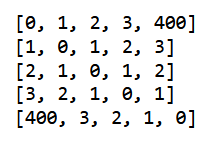
\includegraphics[scale=1]{2947_thesis/pictures/pheromone.png} 
    \caption{Πίνακας pheromone με διαφορετικές επιρροές.}
    \label{15}
\end{figure}
\begin{figure}
    \centering
    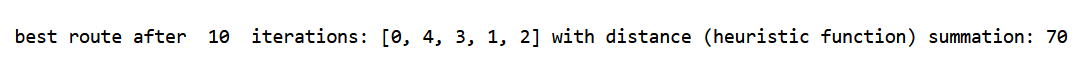
\includegraphics[scale=0.55]{2947_thesis/pictures/ex3.png} 
    \caption{Αποτελέσματα για pheromone [Figure \ref{15}] και beta=0.}
    \label{16}
\end{figure}
Παρατηρούμε ότι τα alpha και beta αποτελούν συμαντικοί παράμετροι για την εύρεση λύσης καθώς επηρεάζουν το πως ο αλγόριθμος βρίσκει την βέλτιστη διαδρομή, αν είναι ιδανικά  για το εκάστοτε πρόβληματα τότε η λύση θα βρεθεί γρηγορότερα. Κατά συνέπεια αν alpha>beta τα μυρμήγκια εστειάζουν στις προηγούμενες λύσεις, δίνοντας έμφαση στην "μνήμη" του προγράμματος, ενώ αν beta>alpha έμφαση δίνετε στην αξία της λύσης την συγκεκριμένη χρονική στιγμή. Κατά συνέπεια η ισορροπία μεταξύ αυτών των δύο παραμέτρων και η σωστή ρύθμιση τους είναι κομβικής σημασίας για την επίτευξη καλών αποτελεσμάτων. 



\subsubsection{Εξασθένιση/Ρυθμός εξασθένισης}
Άλλος ένα σημαντικός παράγοντας για την ορθή εκτέλεση του αλγόριθμου της αποικείας των μυρμηγκιών είναι ο ρυθμός εξασθένισης. Η ρυθμός αυτός βοηθάει στην εξάλειψη των ίχνων φερομόνης σε μη ιδανικά μονοπάτια, που πιθανών οδηγήσουν σε λάθος αποτελέσματα αφού θα αποπροσανατολίσουν τα μυρμήγκια, χωρίς όμως να έχουμε απώλεια πληροφορίας. \cite{mavrovouniotis2014ant}. Ένας υψηλός ρυθμός εξασθένισης (ρ) υποδηλώνει ότι η φερομόνη εξασθενεί ταχύτερα με αποτέλεσμα να παίζει συμαντικότερο ρόλο το κόστος επιλογής κάθε διαδρομής και οι πληροφορίες που σχετίζονται με την φερομόνη από προηγούμενες επαναλήψεις να χάνονται πιο γρήγορα. Δηλαδή, δίνεται περισσότερη βάση στην εξερεύνηση του διαθέσιμου χώρου. Αντίθετα ένας πολύ χαμηλός ρυθμός εξασθένισης (ρ) υποδηλώνει ότι η φερομόνη θα παραμένει στις ακμές περισσότερο χρόνο με αποτέλεσμα τα μυρμήγκια να ακολουθούν τα ίδια μονοπάτια που εξερευνήθηκαν νωρίτερα.
Συνοψίζοντας, υψηλός ρυθμός εξασθένισης δίνει έμφαση στην εξερεύνιση του χώρου ενώ χαμηλός ρυθμός δίνει έμφαση στην "μνήμη" του προγράμματος. Σε περίπτωση που μηδενίσουμε την εξασθένιση παρατηρούμε ότι η σύγκλιση σε βέλτιστη λύση συνήθως καθυστερεί, αυτό συμβαίνει γιατί τα μυρμήγκια τείνουν να επιλέγουν τα ίδια μονοπάτια ακόμα κι αν δεν είναι βέλτιστα. Στο παραδειγμα μας οδηγεί πάλι στην βέλτιστη λύση [Figure \ref{14}] αλλά χρειάζεται (συνήθως) περισσότερο αριθμό επαναλήψεων.


\subsubsection{Επαναλήψεις}
\selectlanguage{greek}Ακόμα ένας σημαντικός παράγοντας για την εύρεση βέλτιστης λύσης είναι ο αριθμός επαναλήψεων (iterations) που θα εκτελεστεί ο αλγόριθμος και τα μυρμήγκια θα ψάξουν για λύση. Θεωρόντας τον πίνακα με την φερομόνη μη ιδανικό \selectlanguage{english}[Figure \ref{pher2}], δοκιμάζουμε τα εξής σενάρια:
\begin{itemize}
    \item iterations=1 [Figure \ref{iter1}]:
    Σε αυτή την περίπτωση, τα μυρμήγκια επηρεασμένα από την φερομόνη ακολουθούν μη βέλτιστη διαδρομή και δεν τους δίνεται χρόνος για εξασθένιση, με αποτέλεσμα να οδηγούμαστε πάντα σε λάθος λύση.
    \item iterations=10 [Figure \ref{iter10}]:
    Αν αυξήσουμε τον αριθμό επαναλήψεων, παρατηρούμε ότι δίνεται χρόνος στα μυρμήγκια να ανακάμψουν από την λάθος διαδρομή και να βελτιωθεί η ποιότητα της λύσης (πολλές φορές και στην βέλτιστη για το παραδειγμα μας), αυτό συμβαίνει αφού δίνεται ο απαραίτητος χρόνος για αντικατάσταση του πίνακα με τις φερομόνες και εξασθένιση της λανθασμένης διαδρομής.
    \item iterations=100 [Figure \ref{iter100}]:
    Αν αυξήσουμε ακόμα περισσότερο τον αριθμό επαναλήψεων, παρατηρούμε ότι τα μυρμήγκια όσες φορές και να εκτελέσουμε τον αλγόριθμο πάντα καταφέρνουν να βρουν την βέλτιστη λύση στο συγκεκριμένο παράδειγμα.
\end{itemize}
\begin{figure}
    \centering
    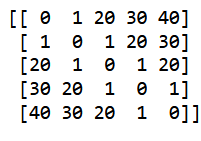
\includegraphics[scale=1]{2947_thesis/pictures/pheromone2.png} 
    \caption{Πίνακας pheromone με διαφορετικές επιρροές.}
    \label{pher2}
\end{figure}
\begin{figure}
    \centering
    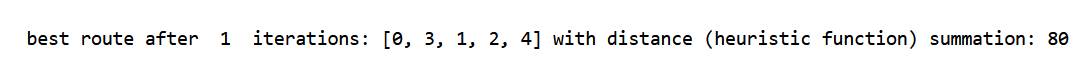
\includegraphics[scale=0.55]{2947_thesis/pictures/ex4.png} 
    \caption{Αποτελέσματα για iterations=1.}
    \label{iter1}
\end{figure}
\begin{figure}
    \centering
    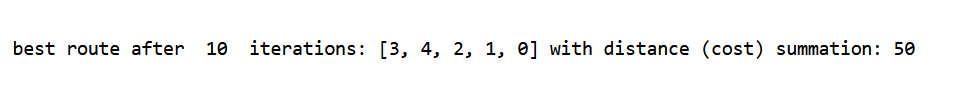
\includegraphics[scale=0.55]{2947_thesis/pictures/ex5.png} 
    \caption{Αποτελέσματα για iterations=10.}
    \label{iter10}

\end{figure}
\begin{figure}
    \centering
    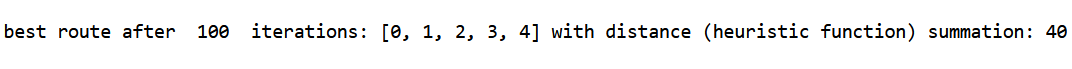
\includegraphics[scale=0.55]{2947_thesis/pictures/ex6.png} 
    \caption{Αποτελέσματα για iterations=100.}
    \label{iter100}
\end{figure}


\subsubsection{Αριθμός μυρμηγκιών}
Ένας ακόμα σημαντικός παράγωντας στον αλγόριθμο μας είναι ο αριθμός των μυρμηγκιών. Αυτός ο αριθμός μπορεί να επηρεάζει σημαντικά την απόδοσή του, μεγάλος αριθμός μυρμηγκιών υποδηλώνει μεγαλύτερο εύρως εξερεύνησης σε λιγότερες επαναλήψεις καθώς και γρηγορότερη σύγκλιση σε μια αποδεκτή λύση, βέβαια αυξάνετε το κόστος σε υπολογιστική ισχύ κάνοντας τον πρόγραμμα πιο αργό στην εκτέλεση του. Αντίστοιχα, μικρός αριθμός μυρμηγκιών μπορεί να όδηγήσει σε πιο αργή σύγκλιση της λύσης στην βέλτιστη, αφού η διαδικασία εξερεύνησης θα είναι πιο χρονοβόρα. Στο παράδειγμά μας, μικρός αριθμός μυρμηγκιών αρκεί για εξερεύνηση των 5 περιοχών, όσο πιο περίπλοκο γίνεται το πρόβλημα, με περισσότερες περιοχές για εξερεύνηση τόσο περίσσοτερα θα πρέπει να είναι και τα μυρμήγκια. 


\subsection{Εφαρμογές Αλγορίθμου}
Ο αλγόριθμος της αποικείας των μυρμηγκιών, όπως ήδη αναφέρθηκε, δίνει λύση σε πληθώρα προβλημάτων του πραγματικού μας κόσμο, όπως είναι η εύρεση βέλτιστης διαδρομή σε προβλήματα δομολόγησης, η βελτιστοποίηση των δικτύων επικοινωνίας, η δρομολόγηση δικτύου δεδομένων και πολλά άλλα. 

\subsubsection{Πρόβλημα του πλανόδιου πωλητή}
Ένα από το πιο μελετημένα προβλήματα που εφαρμόζεται αυτός ο αλγόριθμος είναι αυτό του πλανόδιου πωλητή (Traveling Salesman Problem - TSP), όπου έχει ως στόχο την εύρεση της βέλτιστης διαδρομής που θα περιέρχει όλες τις πόλεις ενός χάρτη ακριβώς μία φορά και θα επιστρέφει στην αρχική πόλη. 

Για την επίτευξη αυτού με χρήση του αλγόριθμου μας, πρέπει να γίνει προσθήκη της επιστροφής του μυρμηγκιού στην αρχική κορυφή και έπειτα εύρεση της βέλτιστης διάδρομή. Εύκολα επιτυγχάνεται αυτό με μια μικρή προσθήκη στον κώδικα. Μετά το βήμα "\#distance sum of the route each ant have chosen" και πριν το "\#the best route of all the chosen ones", γίνεται προσθήκη του "\#returning each ant to its original area", όπως δίνεται παρακάτω:
\lstinputlisting[language=python]{code/update1.py}
Παράδειγμα εκτέλεσης αυτού του αλγορίθμου δίνεται στο [Figure \ref{exret}].
\begin{figure}
    \centering
    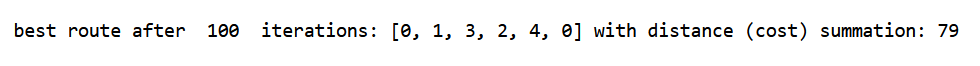
\includegraphics[scale=0.55]{2947_thesis/pictures/ex7.png} 
    \caption{Εκτέλεση με επιστροφή μυρμηγκιού στην αρχική του κορυφή.}
    \label{exret}
\end{figure}

Γίνεται εύκολα κατανοητό ότι το πρόβλημα του πλανόδιου πωλήτη, που ξεκινάει από την πόλη όπου βρίσκεται με στόχο να περάσει όλες τις πόλεις με πελάτη και να γυρίσει στην αρχική το συντομότερο δυνατό επισκέπτοντας κάθε πόλη με πελάτη μόνο μία φορά, ο αλγόριθμος της αποικείας των μυρμηγκιών μπορεί να το προσομοιώσει ικανοποιητικά. 
Αυτό γίνεται αν υποθέσουμε ότι ο γράφος $G=(V(G), E(G))$  που είδαμε παραπάνω αντιπροσωπεύει ένα χάρτη με πόλεις ($V(G)$) και δρόμους ($E(G)$). (Σημείωση ότι εάν το γράφημα δεν είναι πλήρες, δήλαδη δεν υπάρχουν δρόμοι που να ενώνουν όλες τις πόλεις, προσθέτουμε ακμές έτσι ώστε να γίνει με βάρος αρκετά μεγάλο καθιστώντας το απίθανο να επιλεγεί ως βέλτιστη λύση, όπως προτείνεται από Dorigo και Stützle στο \cite{dorigo2004ant}). Σε κάθε δρόμο ($E(G)$) ανατίθεται και ένα κόστος που αντιπροσωπεύει την απόσταση μεταξύ δύο πόλεων (κόστος), αυτό μπορούμε να το προσαρόσουμε ανάλογα με την επιθυμία του πωλητή να ακολουθήσει μία διαδρομή (αν για παραδειγμα ο δρόμος είναι ανηφορικός και είναι με τα πόδια), την κίνηση σε κάθε δρόμο (αν είναι με όχημα) και από πολλούς άλλους παράγοντες. Για λόγους απλότητας θα χρησιμοποιηθεί μόνο η απόσταση. Ο στόχος στο πρόβλημα του πλανόδιου πωλητή είναι η εύρεση του ελάχιστου σε απόσταση κύκλου Hamilton στο γράφο-χάρτη, ένας κύκλος Hamilton είναι ένα μονοπάτι που που επισκέφτεται κάθε πόλη μία φορά και καταλήγει στην αρχική. \cite{dorigo2004ant}

Για την εκτέλεση του αλγορίθμου που υλοποιήθηκε παραπάνω με στόχο την επίλυση του προβλήματος του πλανόδιου πωλητή πρέπει ο πίνακας με το κόστος κάθε διαδρομής (distance) να αντιπροσωπεύει πόλεις και τις αντίστοιχες αποστάσεις μεταξύ τους. 

Διάγραμμα ροής προβλήματος: 





%%%%%%%%%για γράψιμο%%%%%%%%
%Παρουσίαση πρακτικών εφαρμογών γράφων, όπως κοινωνικά δίκτυα, μεταφορές, δρομολόγηση, χαρτογραφία, προβλήματα προσβασιμότητας κ.λπ. Επίδραση της δομής του γράφου στην επίλυση προβλημάτων.
%Data Network Routing \cite{Dorigo-Stützle2},
%routing problems \cite{Dorigo-Stützle2})

